\documentclass{abnt}
\usepackage[a4paper,top=5cm,bottom=2cm,right=4cm,left=2cm,landscape]{geometry}
\usepackage[utf8]{inputenc}
\usepackage[brazil]{babel}
\usepackage{color}

\usepackage{multirow}

\usepackage[pages=some]{background}
\backgroundsetup{
scale=1,
color=white,
opacity=0.15,
angle=0,
contents={%
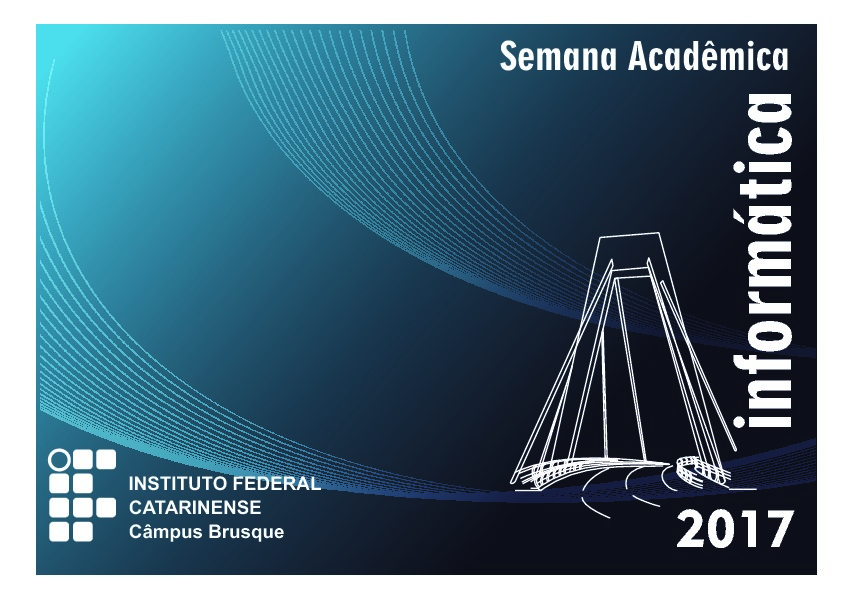
\includegraphics[width=\paperwidth,height=\paperheight]{../imagem-fundo.jpg}}
}

\begin{document}
\BgThispage
\color{black}
\bf
\begin{center}
    \Huge{CERTIFICADO}
\end{center}

Certificamos que Mediador 1, CPF 000.000.000-00, participou da III Semana Acadêmica de Informática do Instituto Federal Catarinense - Campus Brusque, no período de
25/10/2017 a 27/10/2017 como mediador de Discussões sobre o filme 1, perfazendo a carga horária de
00:30 hora(s).

\raggedleft{Brusque, 10 de abril de 2023}

\begin{center}

\includegraphics[scale=0.2]{../assinatura-pb.png}\\
Josiney de Souza\\
Coordenador do Curso Técnico em Informática - Portaria Nº 025/2017\\
Presidente da Comissão Organizadora da III Semana Acadêmica de Informática do Instituto Federal Catarinense - Campus Brusque - Portaria Nº 170/2017
\end{center}

\newpage
\newgeometry{top=1cm,bottom=1cm,left=1cm,right=1cm}
\centering{Programação / Grade de Atividades:}

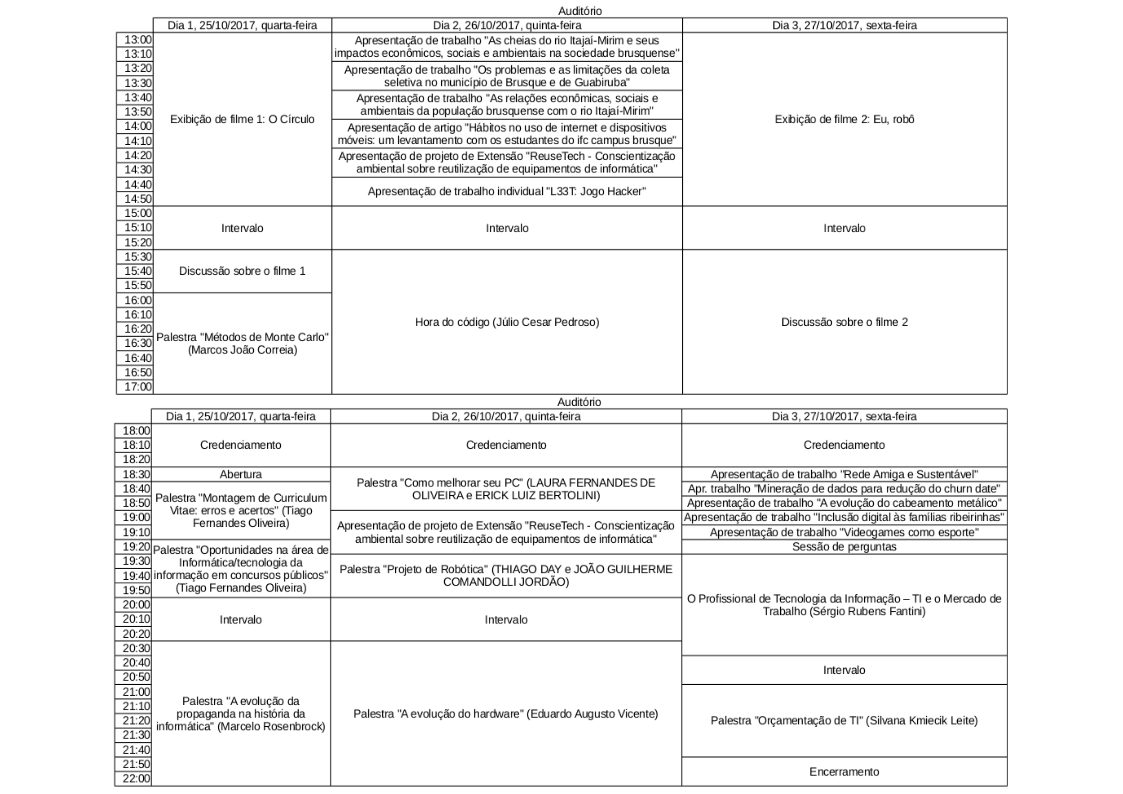
\includegraphics[scale=0.85]{../juncao-grades.png}
\end{document}
